\section{Overall Description}
\subsection{Product Perspective}
\subsubsection{Scenarios}
\begin{enumerate}
    \item \textbf{User wants to start using the eMall service}\\
    The user Matteo decides that he wants to use the eMall service to 
    take advantage of the efficiency it offers. 
    He launches the service and selects the option to sign up. 
    Matteo then inputs all the relevant information and he is granted access to the service.
    \item \textbf{User books the recharge for his car}\\
    After a long drive, the user Matteo noticies that the level of his battery is low. 
    He stops, takes his phone and launches the eMall service, logs in, and then he is presented with all the nearby stations.
    He then selects a specific timeslot for charging and he is presented with all the available nearby stations.
    He selects a station, views all the station's information and then chooses a station according to his preferences and then finalizes the booking.
    The user then receives the socket's identification.
    \item \textbf{User starts the charge}\\
    The user Matteo drives to a station that he has a charge booked with, he then unlocks the booked socket from the service, he then connects his electric 
    vehicle to the socket and, after he has left the vehicle, he launches the eMall service and 
    he is presented with the option to start the vehicle's charge. He selects this option and the station initiates charging on the booked socket. eMall than shows the user the estimated time for the full charge of the vehicle. 
    \item \textbf{User is notified of a finished charge}\\
    After the user Matteo has started to charging process at the station,
     he goes to a nearby cafeteria to have a cup of coffee. When the car has fully charge, the eMall service notifies him on his phone with a push notification.
    \item \textbf{User pays for the service}\\
    The user Matteo, after he has used the eMall service for a successful charge, provided that he has not paid for the service yet,
    launches the app and he is presented with the option to pay for the service, 
    he selects this option and then enters his credit card information.
    The service that processes his payment, and if it is successful he is presented with a success message.
    \item \textbf{User is reminded to charge his electric vehicle}\\
    While the user Matteo is driving, the eMall service monitors the car's battery level, the user's location and his schedule. 
    When the service finds an optimal place to charge, related to schedule, location and state of charge it notifies the user with a push notification.
    Matteo then stops, launches the eMall service and then he is presented with the optimal station to charge, based on his location, the best timeslot with respect to his schedule and the stations' prices. He then books the charge.
\end{enumerate}
\subsubsection{Class Diagram}

%\subsubsection{State Diagrams}
\subsection{Product Functions}
In this section the main functionalities of eMall are presented and described.
\subsubsection{Sign up}
This functionality lets the registration of \textbf{Users}(\ref{Users})  in order to use eMall. The first step is to enter the registration form, then the User inserts his credentials; if correct an e-mail is sent to the inserted address and it is required to validate it. 
Finally the User is taken to the login page.
\begin{figure}[H]
    \begin{center}
        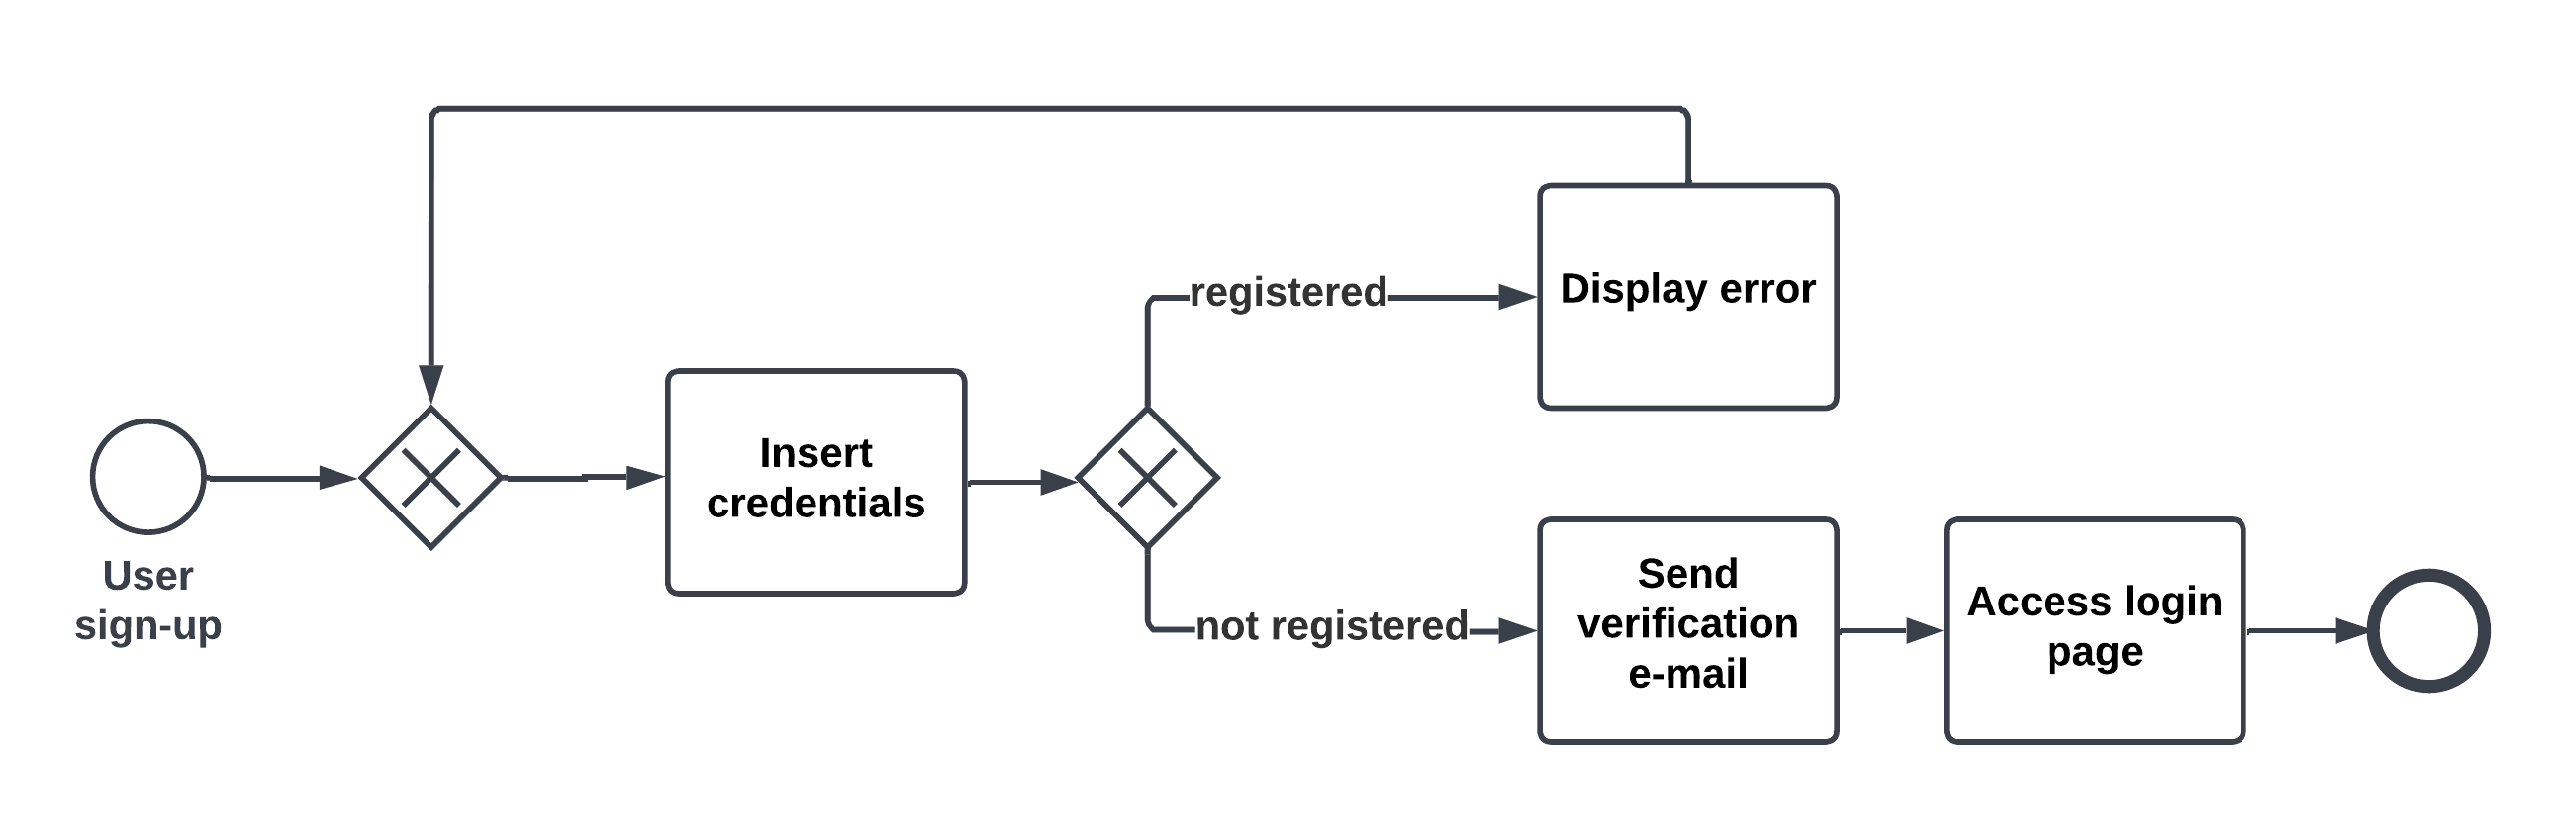
\includegraphics[width=\textwidth]{img/fun-sign-up.png}
        \caption{BPMN diagram sign up method}
    \end{center}
\end{figure}
\subsubsection{View the nearby charging stations}
This functionality allows the \textbf{Users}(\ref{Users}) to view information about the nearby charging stations, and is available to all of the logged Users. 
The first step is to open the eMall service and the User is presented with the nearby charging stations. 
If he clicks on one of the stations, the user can view the current station's recharge price and socket availability.
The User at any time can go back to view the other stations and he is free to view information about them.\label{View}
\begin{figure}[H]
    \begin{center}
        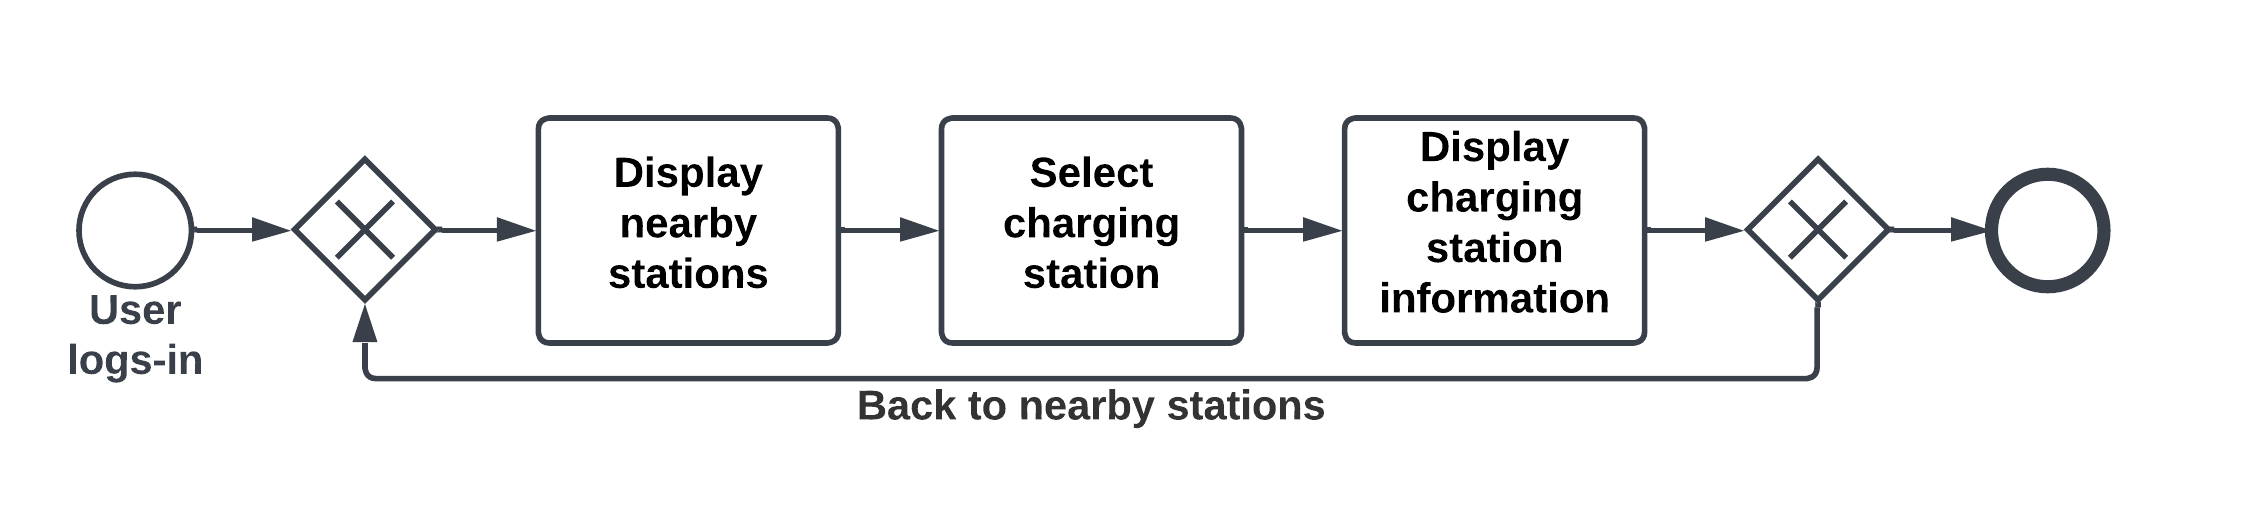
\includegraphics[width=\textwidth]{img/fun-view-info.png}
        \caption{BPMN diagram view nearby stations method}
    \end{center}
\end{figure}
\subsubsection{Charge booking}
This functionality allows the \textbf{Users}(\ref{Users}) to book a charge for their electric vehicle, and is available to all of the logged Users. 
The first step is to open the eMall service and to select a preferred timeslot for charging. The second step is to pick a station from the stations view (As described in \ref{View}).
Finally, the User can select the "Book" option to reserve his timeslot at the selected station for charging.
He then is presented with a brief summary of the booking, like the socket's identification and the station's address.
He can also view the summary at anytime in a specific section of the service.\label{Book} 
\begin{figure}[H]
    \begin{center}
        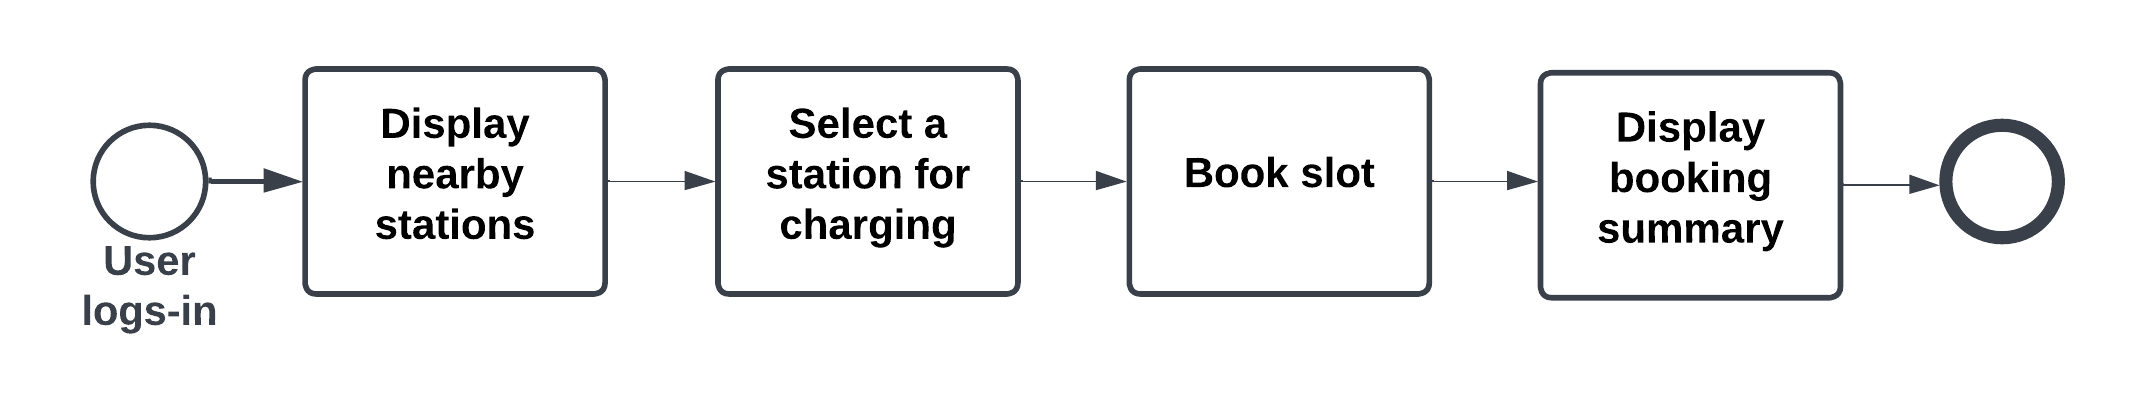
\includegraphics[width=\textwidth]{img/fun-book-slot.png}
        \caption{BPMN diagram charge booking method}
    \end{center}
\end{figure}
\subsubsection{Remotely unlocking a socket}
This functionality allows the \textbf{Users}(\ref{Users}) to unlock a charging socket to charge their electric vehicle, and is available when a logged User has booked a recharge at a station. 
The User must access the brief summary of his booking (As described in \ref{Book}).
He can select the "Unlock" option to unlock his booked socket, in order to connect his car to the socket.
\begin{figure}[H]
    \begin{center}
        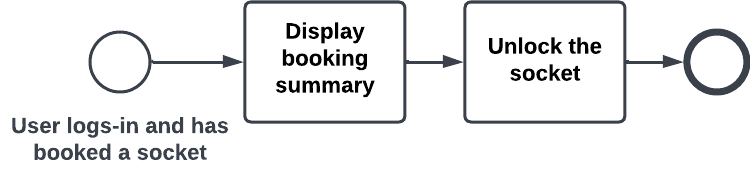
\includegraphics[scale=0.3]{img/fun-sock-unl.png}
        \caption{BPMN diagram socket unlocking method}
    \end{center}
\end{figure}
\subsubsection{Remotely starting a charge}
This functionality allows the \textbf{Users}(\ref{Users}) to remotely start the charge for their electric vehicle, and is available when a logged User has booked a recharge at a station, and has connected his car to the socket. 
The User must access the brief summary of his booking (As described in \ref{Book}).
He can select the "Start charging" button to remotely start the charging process on his booked socket.
\begin{figure}[H]
    \begin{center}
        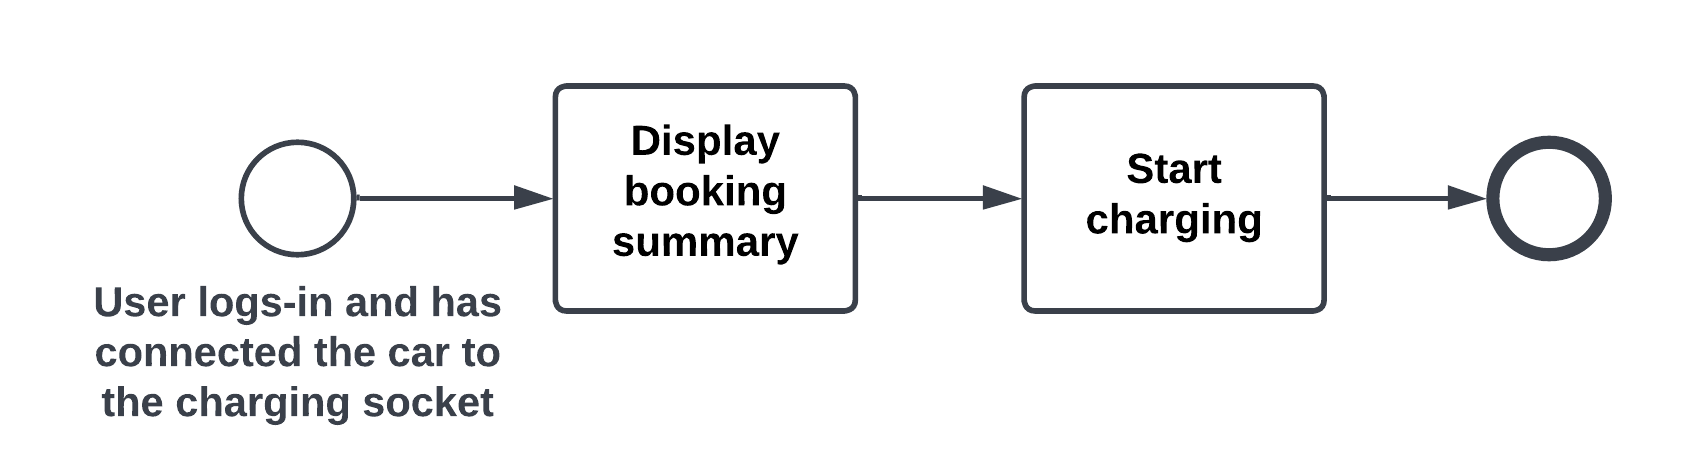
\includegraphics[scale=0.2]{img/fun-rem-ch.png}
        \caption{BPMN diagram remotely starting the charge method}
    \end{center}
\end{figure}
\subsubsection{Notify of a finished charge}
This functionality allows the \textbf{Users}(\ref{Users}) to be informed when the charging process has finished, and is available when a logged User has been charging his car at a station.
When the charging process ends, the user is notified (with a push notification) that his car is fully charged.
\begin{figure}[H]
    \begin{center}
        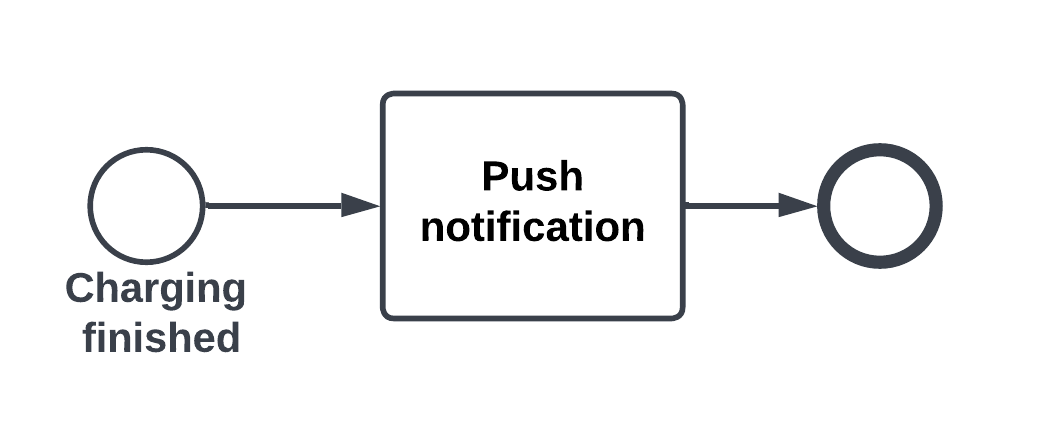
\includegraphics[scale=0.2]{img/fun-not-fin.png}
        \caption{BPMN diagram notify a finished charge method}
    \end{center}
\end{figure}
\subsubsection{Pay for the service}
This functionality allows the \textbf{Users}(\ref{Users}) to pay for the charging service, provided that he has used the service.
When the charging process ends, the User can open the brief summary of his reservation (As described in \ref{Book}) in order to pay for the service.
After the opens the summary, he is presented with the option to pay and if it picked, he should enter his credit card's information and click the "Submit" button.
If the payment has been successful, the service shows him the success screen and the summary of the reservation will be marked as paid, otherwise he is returned to enter a valid credit card's information.
\begin{figure}[H]
    \begin{center}
        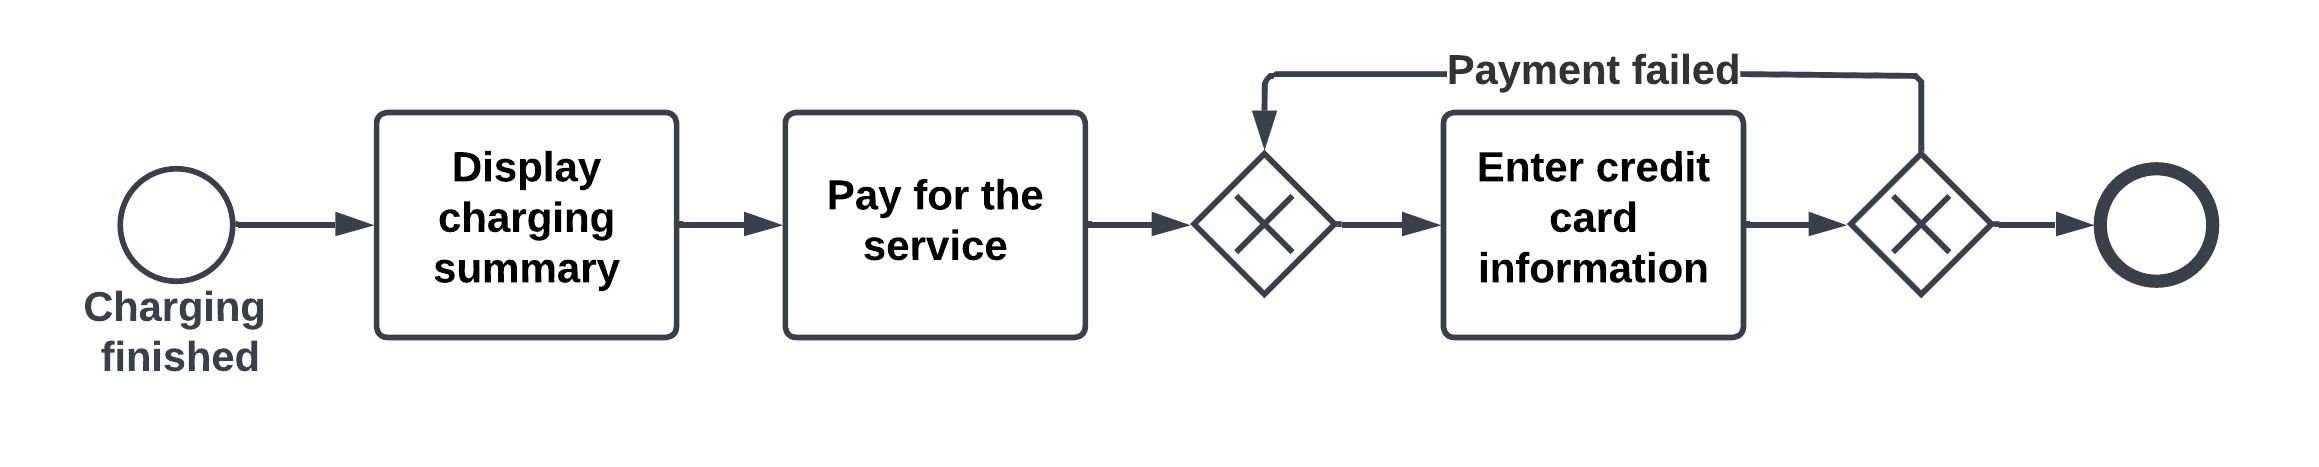
\includegraphics[width=\textwidth]{img/fun-pay.png}
        \caption{BPMN diagram pay for the service method}
    \end{center}
\end{figure}
\subsubsection{Send suggestions}
This functionality allows the \textbf{Users}(\ref{Users}) to receive optimal suggestions for charging.
The system continously monitors a user's charging level, his schedule and his location.
The system has an internal model to determine an optimal place to charge if battery level is under 50\%, based on location and schedule.
When it determines an optimal place and timeslot, the model will also determine the optimal time to suggest the user.
The user will than be notified at the computed time with a push notification. The notification will contain the optimal place to charge and an optimal timeslot, with maximum compatibility with the user's lifestyle. 
\begin{figure}[H]
    \begin{center}
        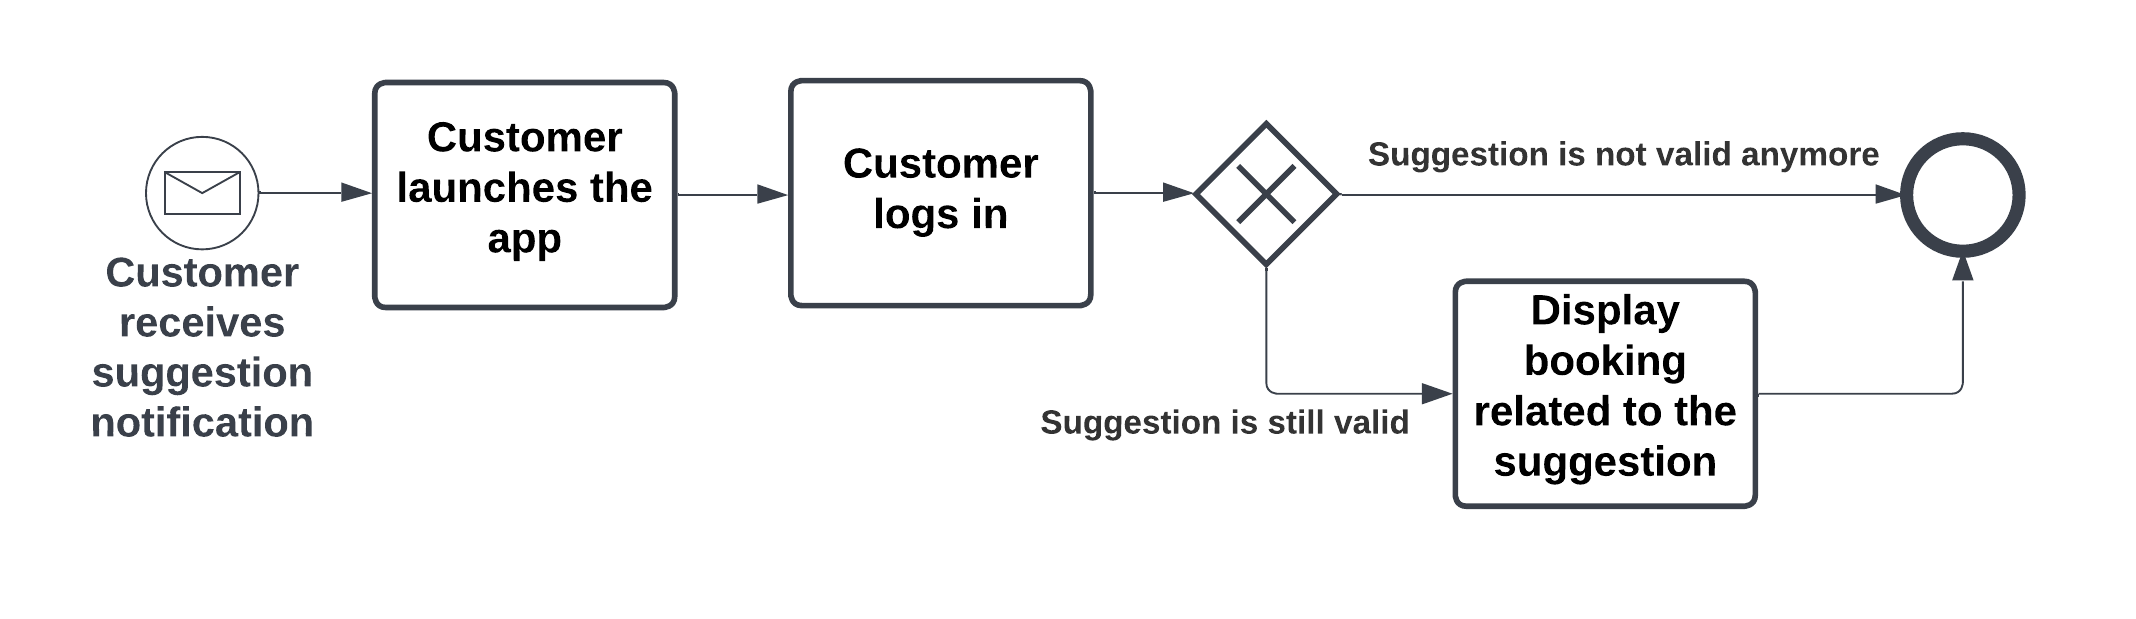
\includegraphics[width=\textwidth]{img/fun-sug.png}
        \caption{BPMN diagram send suggestions method}
    \end{center}
\end{figure}
%
\subsection{User Characteristics}
The following three actors are considered in the e-Mall system.
\subsubsection{Unregistered User}
It's a person that doesn't have a registered account in the e-Mall application. 
In this case, he can register an account to use the platform.
\subsubsection{Registered User}
It's a person that has a registered account in the e-Mall application. 
He is able to use the e-Mall service and book a charge for his electric vehicle through the service.
He is also able to unlock a charging socket for his reservation and to pay for the service through the platform.
\subsubsection{e-Mobility Service Provider}
It's a company that offers the vehicle charging service. It offers all its services though the e-Mall platform.
eMSPs rely on multiple Charging Point Operators for actual charging process.
\subsubsection{Charging Point Operator}
It's the charging station owner and manager. This actor is responsible for the supply of the charging service offered by eMSPs. 
Every reservation made on the e-Mall platform is fulfilled by CPOs.
\subsubsection{Distribution System Operator}
This actor is represented by the companies that supply energy to CPOs.
\subsection{Assumptions, Dependencies and Constraints}
\subsubsection{Assumptions}
\begin{enumerate}[label=\textbf{D\arabic*}:]
    \item Each user who wants to use the online service is needed to have a device connected to Internet (such as PC, Mac, smartphone, etc).
    \item The user's mobile device fully supports the push notification technology.
    \item The user's schedule and location is accessible by the platform.
    \item The charging station checks the charging sockets, making sure that nobody can occupy a reserved socket apart from the booker.
    \item The data automatically obtained by the system in order to send suggestions to the user is accurate and truthful.
    \item Every CPMS system has the same communication methods. (Uniform APIs)
    \item A generic CPMS system has to offer the following functions:
        \begin{itemize}
            \item Expose the information about the status and data of every charging station socket. (e.g. availability, type of socket, cost, time for the first socket to be free)
            \item Start a charge on a specific socket.
            \item Monitor the charge on a specific socket.
            \item Infer at what time the charging process will be finished.
        \end{itemize}
    \item A fully functioning payment system is present and returns if a transaction has been successful or not.
    \item ?? come fa la stazione di ricarica a capire che è occupata?
    \item Every station has at least one charging socket.**
    \item Every eMSP must interact with at least one CPO.**
\end{enumerate}